\documentclass[12pt,oneside,final]{thesis}

\usepackage[superscript]{cite}
\usepackage{amsmath,amsfonts}
\usepackage{graphicx}
\graphicspath{{./figs/}}
\usepackage{fixltx2e}
\usepackage{array}
% wrapfig is fragile: use sparingly
\usepackage{wrapfig} 
%\usepackage{times}  % Use this for ugly fonts

\usepackage{upgreek}
\usepackage{hyperref}
\usepackage{setspace}

\usepackage{booktabs}
\usepackage{multirow}
\usepackage{longtable}
\usepackage[font=singlespacing, labelfont=bf]{caption}
%\usepackage{CV}

\usepackage{enumitem}
\newlist{inlinelist}{enumerate*}{1}
\setlist*[inlinelist,1]{%
  label=(\arabic*),
}

\usepackage{fancyhdr}    % Use nice looking headers along with the required footer page numbers   
%\usepackage[hypertex]{hyperref}

%Define the header/footer style
\pagestyle{fancy}
\fancyhf{}
\setlength{\headheight}{15pt}
\lhead{\leftmark}
\cfoot{\thepage}
\renewcommand{\headrulewidth}{0pt}
\fancypagestyle{plain}{% Redefine ``plain'' style for chapter boundaries
\fancyhf{} % clear all header and footer fields
\fancyfoot[C]{\thepage} % except the center
\renewcommand{\headrulewidth}{0pt}
\renewcommand{\footrulewidth}{0pt}}

%\tolerance=10000

%\makeglossary % enable the glossary

\begin{document}

\title{JHU THESIS TEMPLATE}
\author{R. Jacob Vogelstein}
\degreemonth{May}
\degreeyear{2007} 
\dissertation
\doctorphilosophy
\copyrightnotice


% add your chapters, best way is to have separate TeX files for each chapter
%% FRONTMATTER
\begin{frontmatter}

% generate title
\maketitle

\begin{abstract}

Abstract goes here.

\vspace{1cm}

\keywords{Consumption, Marginal Propensity to Consume, Heterogeneity}

\JEL{D12}

\Advisors{\\ Professor Christopher Carroll\\ Professor Jon Faust\\ Professor Jonathan Wright}


\end{abstract}

\begin{acknowledgment}

Thanks!

\end{acknowledgment}

\begin{dedication}
 
This thesis is dedicated to \ldots

\end{dedication}

% generate table of contents
\tableofcontents

% generate list of tables
\listoftables

% generate list of figures
\listoffigures

\end{frontmatter}

\chapter{Introduction}
\label{sec:intro}
\chaptermark{Optional running chapter heading}

Introduction.

A citation \cite{A}. 
A citation without brackets \citen{B}. 
Multiple citations \cite{A, B, C}.

\section{Section}
\label{sec:section}

This is a section.  Here's a reference to a different section:
\ref{sec:subsection}.

\subsection{Subsection}
\label{sec:subsection}

This is a subsection.

% \begin{figure}[t]
% \centering
% \includegraphics[width=\textwidth]{figure}
% \makeatletter
% \let\@currsize\normalsize
% \caption{Caption.}
% \label{fig:figure}
% \end{figure}
% 
% \begin{figure}[t]
% \centering
% \begin{tabular}{c c}
% \includegraphics[height=2.5in]{figureA} &
% \includegraphics[width=3in]{figureB}\\
% (A) & (B)
% \end{tabular}
% \makeatletter
% \let\@currsize\normalsize
% \caption{Two figures.}
% \label{fig:twofigures}
% \end{figure}

% currsize is not set in the long table environment, so we need to set it before we set it up.
\makeatletter
\let\@currsize\normalsize
\makeatother

% tabular environments are set to be single-spaced in the  thesis class,  but long tables do not use tabular
% to get around this, set the spacing to single spacing at the start of the long table environment, and set it back to double-spacing at the end of it
\ssp
\begin{longtable}{cc}
\caption[This is what I want to have in the LOT]{This is a caption.} \label{tab:pfams} \\
\hline
A & B \\
\hline
\endfirsthead
\multicolumn{2}{@{}l}{\textbf{Table \thetable} \ldots continued} \\
\hline
A & B \\
\hline
\endhead
a1 & b1 \\
a2 & b2 \\
a3 & b3 \\
a4 & b4 \\
\hline
\end{longtable}
\dsp

\section[Optional table of contents heading]{Section with\\linebreaks in\\the
name}

This is another section.

\subsection{Another subsection}

\subsubsection{Subsubsection}

\paragraph{Heading level below subsubsection}
\label{sec:paragraph}

And I quote: 
%
\begin{quote}
La la la.
\end{quote}
%
\noindent No ident after end of quote.  

Another paragraph with a list:
%
\begin{itemize}
%  
\item Item 1
%
\item Item 2
%
\end{itemize}
%
\noindent Again, we don't indent here.

\include{appendix}

%% REFERENCES

% if you use BIBTEX
\bibliographystyle{IEEEtran}
\bibliography{thesis}

\begin{vita}

\begin{wrapfigure}{l}{0pt}
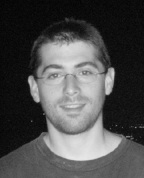
\includegraphics[width=2in,height=2.5in,clip,keepaspectratio]{rjvheadshot}
\end{wrapfigure}

R.\ Jacob Vogelstein received the Sc.\ B.\ degree in Bio-Electrical Engineering 
from Brown University in 2000,  and enrolled in the Biomedical Engineering 
Ph.D.\ program at Johns Hopkins University in 2001.  He was inducted into the 
Tau Beta Pi and Sigma Xi honor societies in 1999, won the Brown University 
Engineering Department's Outstanding Student Award in 2000, and received a 
National Science Foundation Graduate Research Fellowship in 2002.  His research 
focuses on neuromorphic and neuroprosthetic devices, and his papers have been 
finalists in the student paper competitions at the 2004 IEEE International 
Conference of the Engineering in Medicine and Biology Society and the 2004 IEEE 
International Conference on Electronics, Circuits and Systems.

Starting in June 2007, Jacob will work on the ``Revolutionizing Prosthetics 2009'' 
project at the Johns Hopkins University Applied Physics Laboratory in Laurel,
MD, where he will help to create the next-generation of upper-arm
neuroprostheses.  

\end{vita}
\end{document}